\section{Web Interface}
\label{sec:web-interface}
	In order illustrate the system's functionality, a web-based interface was created.  It provides users with a simple way to interact with the system.
	
	The first step involves searching for entities by a value.  We use approximate (\(n\)-gram) string matching to find relevant values despite potential character substitutions, deletions, or additions.  Users are presented with a list of candidate values to choose from, as seen in \cref{fig:webui-step-1}.
	
	\begin{figure}[H]
		\centering
		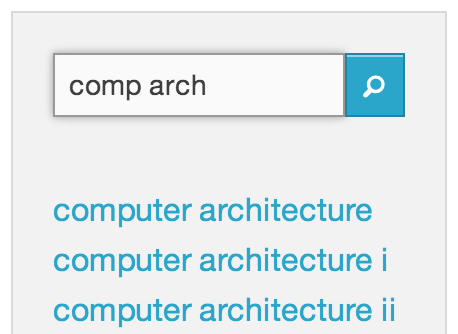
\includegraphics[scale=0.5]{figures/images/step-1}
		
		\caption{Approximate string matching of values}
		\label{fig:webui-step-1}
	\end{figure}
	
	Entities that match the desired values are displayed to the user (\cref{fig:webui-step-2}).  They have the option of specifying the entity as either the source, or the target.  The source and target are the two entities the user wishes to connect.
	
	\begin{figure}[H]
		\centering
		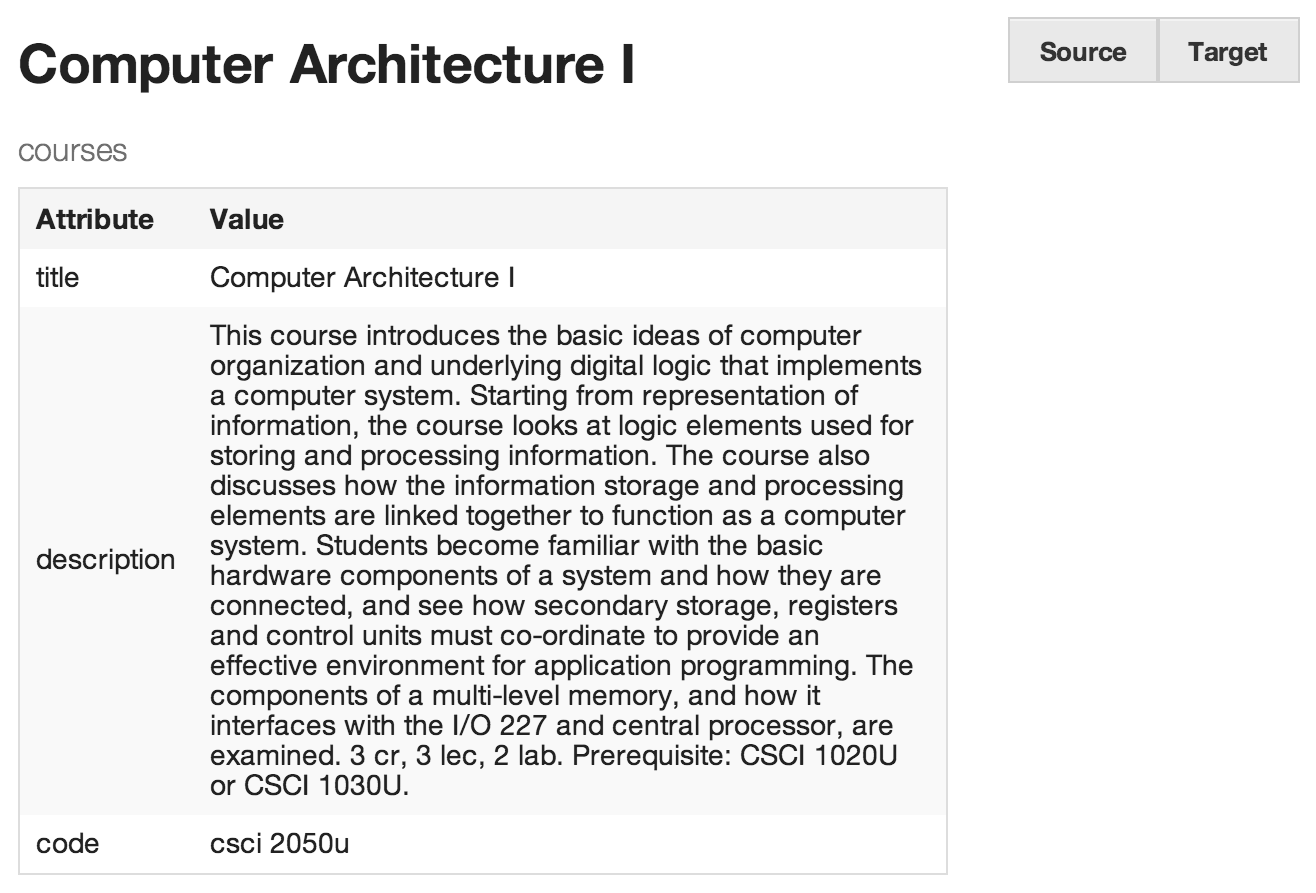
\includegraphics[scale=0.5]{figures/images/step-2}
		
		\caption{Tabular display of entities}
		\label{fig:webui-step-2}
	\end{figure}
	
	When an entity is chosen, the navigation bar at the top of the page is updated to reflect the new selection (\cref{fig:webui-step-3}).  This allows the user to hover their cursor over the respective element to remind themselves of their selection.
	
	\begin{figure}[H]
		\centering
		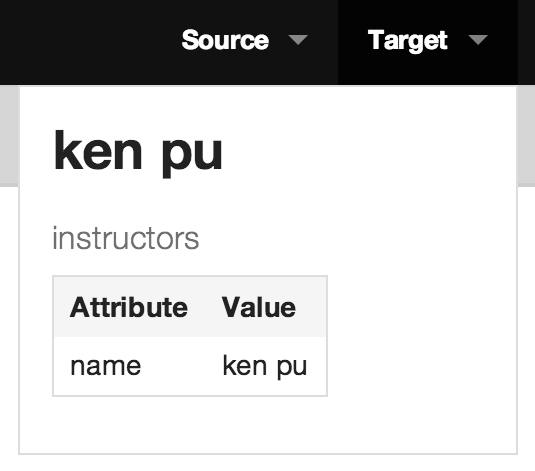
\includegraphics[scale=0.5]{figures/images/step-3}
		
		\caption{Chosen entities are displayed at the top}
		\label{fig:webui-step-3}
	\end{figure}
	
	When both a source and target entity are selected, the user is able to search for the shortest path between them.  They are given the option of which graph search algorithm implementation to use, as seen in \cref{fig:webui-step-4}.
	
	\begin{figure}[H]
		\centering
		
\includegraphics[scale=0.5]{figures/images/step-4}
		
		\caption{The algorithm implementation may be selected}
		\label{fig:webui-step-4}
	\end{figure}
	
	A short message displaying the search duration as well as memory consumption is followed by a series of tables representing the intermediate entities between the source and target entities (\cref{fig:webui-step-5}).
	
	\begin{figure}[H]
		\centering
		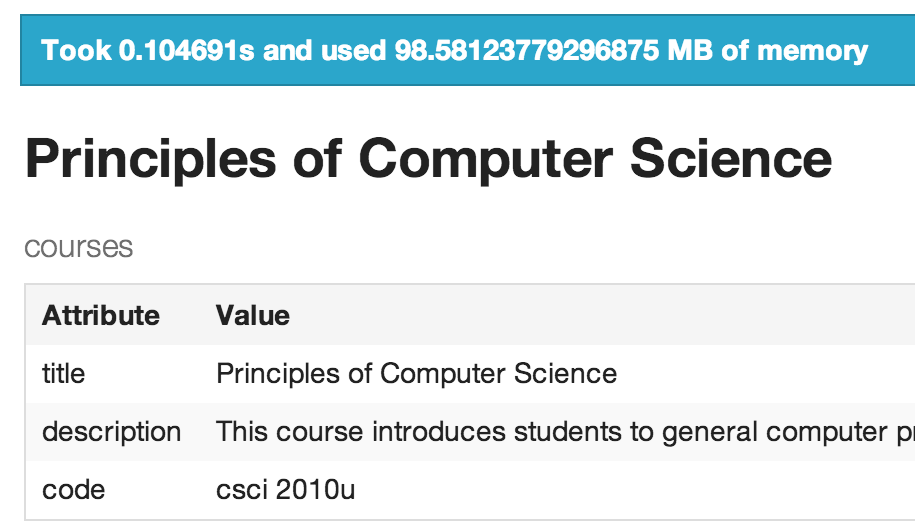
\includegraphics[scale=0.5]{figures/images/step-5}
		
		\caption{Result of a search between entities}
		\label{fig:webui-step-5}
	\end{figure}